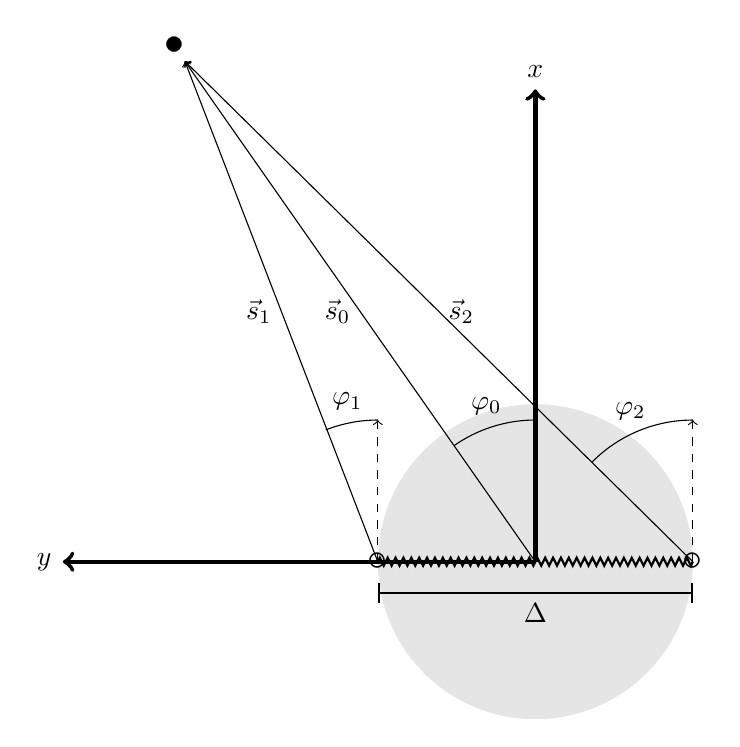
\begin{tikzpicture}[scale=4]
% Parameters
\def\radius{1.5};
\def\arrowScale{0.97};

\def\micSpacing{1};
\def\micL{-0.5*\micSpacing};
\def\micR{0.5*\micSpacing};

\def\sourceRadius{2};
\def\sourceAzimuth{35}
\pgfmathsetmacro\sourceY{cos(-\sourceAzimuth)*\sourceRadius}
\pgfmathsetmacro\sourceX{sin(-\sourceAzimuth)*\sourceRadius}

\pgfmathsetmacro\sourceLAzimuth{-atan((\sourceX-\micL)/\sourceY)}
\pgfmathsetmacro\sourceRAzimuth{-atan((\sourceX-\micR)/\sourceY)}

\def\arcRadius{0.45};
\pgfmathsetmacro\arcY{cos(-\sourceAzimuth/2)*\arcRadius}
\pgfmathsetmacro\arcX{sin(-\sourceAzimuth/2)*\arcRadius}
\pgfmathsetmacro\arcLY{cos(-\sourceLAzimuth/2)*\arcRadius}
\pgfmathsetmacro\arcLX{sin(-\sourceLAzimuth/2)*\arcRadius}
\pgfmathsetmacro\arcRY{cos(-\sourceRAzimuth/2)*\arcRadius}
\pgfmathsetmacro\arcRX{sin(-\sourceRAzimuth/2)*\arcRadius}

% Coordinate system
\draw[ultra thick,->] (0,0) -- (0,\radius) node[above]{$x$};
\draw[ultra thick,->] (0,0) -- (-\radius,0) node[left]{$y$};

% Arrows
\node at (\sourceX,\sourceY){\Large $\bullet$}; % source
\draw[->] (0,0) -- (\arrowScale*\sourceX,\arrowScale*\sourceY) node[left, pos=0.5]{$\vec{s}_0$}; % origin
\draw[->] (\micL,0) -- (\arrowScale*\sourceX,\arrowScale*\sourceY) node[left, pos=0.5]{$\vec{s}_1$}; % left mic
\draw[->] (\micR,0) -- (\arrowScale*\sourceX,\arrowScale*\sourceY) node[right, pos=0.5]{$\vec{s}_2$}; % right mic
\draw[thick, decoration = {zigzag, segment length = 1mm, amplitude = 0.5mm}, decorate] (\micL,0) -- (\micR,0); % navigable region

% Arcs
\draw[domain=90:(90+\sourceAzimuth)] plot ({\arcRadius*cos(\x)}, {\arcRadius*sin(\x)});
\node at (1.15*\arcX,1.15*\arcY){$\varphi_0$};

\draw[dashed,->] (\micL,0) -- (\micL,\arcRadius); % left mic
\draw[domain=90:(90+\sourceLAzimuth)] plot ({\arcRadius*cos(\x) + \micL}, {\arcRadius*sin(\x)});
\node at (1.15*\arcLX + \micL,1.15*\arcLY){$\varphi_1$};

\draw[dashed,->] (\micR,0) -- (\micR,\arcRadius); % right mic
\draw[domain=90:(90+\sourceRAzimuth)] plot ({\arcRadius*cos(\x) + \micR}, {\arcRadius*sin(\x)});
\node at (1.15*\arcRX + \micR,1.15*\arcRY){$\varphi_2$};

% Mic positions
\node at (\micL,0){\Large $\circ$};
\node at (\micR,0){\Large $\circ$};
\draw[thick,|-|] (\micL,-0.1) -- (\micR,-0.1) node[below, pos=0.5]{$\Delta$};

\fill [color=black,opacity=0.1] (0,0) circle (\micSpacing/2);

\end{tikzpicture}